\chapter{Implementación de sistema de inferencia y extensión para ambientes de desarrollo}
En esta sección se detalla la implementación de la propuesta de solución, y se divide en dos componentes principales. Primero, se implementó un sistema de inferencia para la desclasificación basada en tipos en el lenguaje de programación Dart. Segundo, se elaboró una extensión para ambientes de desarrollo que soportan servidores de análisis estático de Dart, que integra el resultado de la inferencia.

\section{Librerías utilizadas}
La implementación de este trabajo fue realizada en Dart, debido a que los investigadores que realizaron el trabajo de la desclasificación basada en tipos estudian este lenguaje como parte de un proyecto de investigación mayor en el área de seguridad. A continuación se nombran las librerías de Dart utilizadas en el desarrollo de este trabajo.

\subsection{Dart Analyzer}
\emph{Dart Analyer} es una herramienta incluida en Dart, que permite realizar análisis estático de código Dart. Entre otros servicios, esta herramienta permite obtener el AST de un código Dart. Dicho AST contiene la información relevante del programa, incluyendo el resultado del análisis de tipos.

Análisis personalizados de programas en Dart pueden ser realizados usando la información del AST. Dart Analyzer utiliza el patrón Visitor para incorporar un nuevo análisis sobre el AST, y así facilitar su integración con otros análisis.

\subsection{Analyzer Plugin}
La herramienta \emph{Analyzer Plugin} sirve para integrar un análisis personalizado sobre el AST generado por Dart Analyzer, con los ambientes de desarrollo que tengan soporte para servidores de análisis estático de Dart, como IntelliJ, Eclipse, Atom, entre otros.

Un plugin de Dart Analyzer se implementa en Dart, y utiliza una API para comunicarse con el servidor de análisis. La API consiste en tres tipos de comunicación:

\begin{enumerate}
  \item Cuando el servidor de análisis necesita enviar información al plugin, o necesita pedir información al plugin, envía un \emph{request}.
  \item El plugin responde a toda request del servidor de análisis con un \emph{response}.
  \item El plugin puede enviar \emph{notificaciones} al servidor de análisis con información.
\end{enumerate}

Mediante el envío de notificaciones o respondiendo a peticiones del servidor de análisis, el plugin puede enviar información respecto a errores, resaltado de sintaxis, sugerencias de navegación, sugerencias de edición y marcado de ocurrencias, las cuales serán desplegadas en la interfaz del IDE.

\section{Implementación de sistema de inferencia}

\subsection{Representación de facetas públicas}
Para declarar las facetas públicas, se usan las anotaciones de Dart. Por ejemplo,

 \texttt{@S("Bot") bool check(@S("StringCompareTo") String password);}

 es una declaración de un método de Dart anotado con facetas públicas. Este método declara una faceta pública \texttt{Bot} como retorno, y una faceta pública \texttt{StringCompareTo} para el parámetro \texttt{password}, que fue definida previamente. Cuando se declara una faceta pública \texttt{@S("Bot")}, se refiere a una faceta pública con todos los métodos que tiene la faceta privada.

La definición de las facetas públicas se hace mediante clases abstractas de Dart. Por ejemplo, la faceta \texttt{StringCompareTo} se define mediante la clase abstracta del mismo nombre:
\vspace{0.5em}
\begin{lstlisting}
  abstract class StringCompareTo {
    int compareTo(String other);
  }
\end{lstlisting}

Antes de la generación de restricciones sobre un archivo, se realiza una etapa de \textit{parsing} de facetas públicas, en donde se leen las clases abstractas del archivo. Esto se implementa mediante el \emph{visitor} \texttt{DeclaredFacetVisitor}, que se muestra en el diagrama de la figura \ref{uml}. Las facetas públicas procesadas se almacenan en el diccionario \texttt{declaredStore}, en donde se asocia el nombre de la faceta con su tipo de objeto correspondiente.

\subsection{Fase de generación de restricciones}
Una vez que se procesan las facetas públicas, se procede a la generación de restricciones. Esto se realiza implementando varios visitors mostrados en el diagrama de la figura \ref{uml}.

La clase encargada de procesar las clases declaradas en un archivo es \texttt{CompilationUnitVisitor}. Mediante el visitor \texttt{ClassMemberVisitor}, se procesa cada método, campo y constructor de cada clase. Finalmente, el visitor implementado para procesar el cuerpo de cada miembro es \texttt{BlockVisitor}, en donde se procesa cada expresión relevante para el algoritmo de generación de constraints de la sección \ref{propuestaGen}.

La clase \texttt{Store} es la encargada de la generación de variables de tipo, y el almacenamiento en diccionarios del tipo de las expresiones y elementos. Una expresión es un ente sintáctico representado por un nodo en el AST, mientras que un elemento es un ente semántico que fue declarado con un nombre en algún lugar del programa.

Por ejemplo, el nodo \texttt{MethodInvocation} representa una expresión de invocación a método. Desde este nodo es posible obtener un \texttt{MethodElement}, que representa la declaración del método invocado.

El diccionario que almacena el tipo de las expresiones es necesario para almacenar información que no es posible acceder desde nodos que la necesitan. Por ejemplo, en el nodo \texttt{ReturnStatement} se genera una restricción entre la expresión de retorno y el retorno del método. La expresión de retorno es un hijo del nodo \texttt{ReturnStatement}, por lo que debe ser visitado antes de generar la restricción, para que guarde el tipo de la expresión en el diccionario y pueda ser obtenido en el nodo padre.

El diccionario que almacena el tipo de los elementos es necesario para la generación de restricciones sobre identificadores. Por ejemplo, en una invocación a método sobre una variable, se debe obtener el tipo del \texttt{VariableElement} para generar la restricción de invocación a método. Además, al final del proceso de inferencia, los elementos incluidos en este diccionario deben ser marcados en el código fuente para informar el tipo inferido al programador.

En la fase de generación de restricciones se pueden generar errores de tipo \texttt{IllFormedTypeError} y \texttt{UndefinedFacetWarning}, los cuales son recolectados mediante un \texttt{ErrorCollector}, el cual será utilizado para el despliegue de la información mediante la extensión.
\clearpage
\begin{figure}[ht]
  \centering
  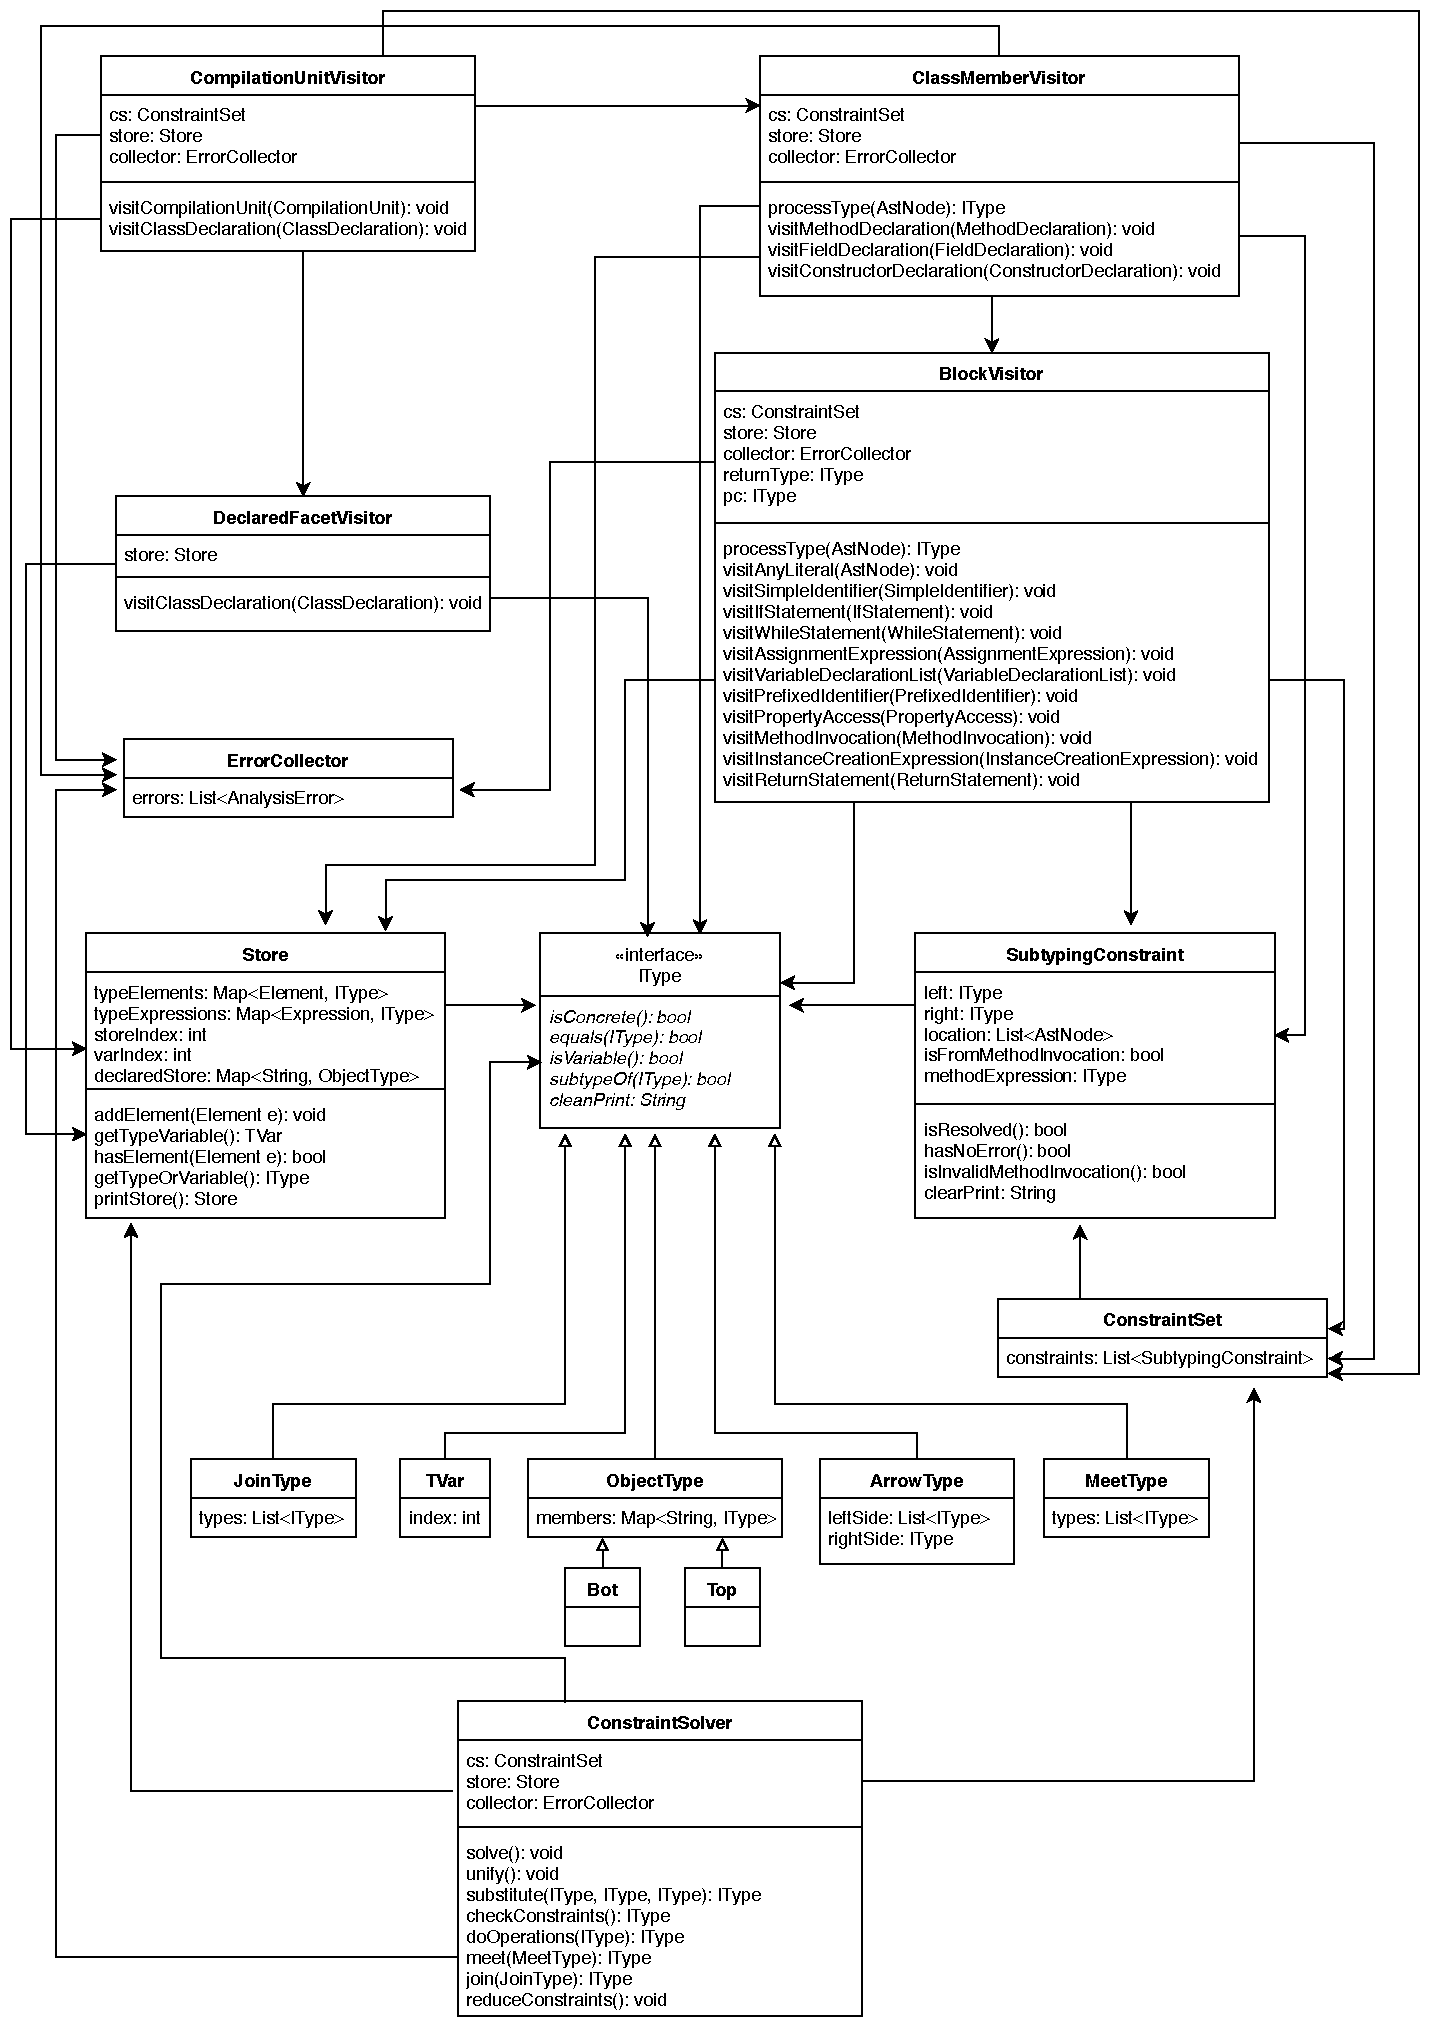
\includegraphics[width=0.93\textwidth]{imagenes/others.pdf}
  \caption{Diagrama de clases de sistema de inferencia}
  \label{uml}
\end{figure}
\clearpage
\subsection{Fase de resolución de restricciones}
En esta fase, la clase \texttt{ConstraintSolver} se encarga de convertir el conjunto de restricciones en un mapeo entre variables de tipo y tipos concretos, implementando las operaciones descritas en la sección \ref{propuestaRes}. Esta clase se muestra en el diagrama \ref{uml}.

En el algoritmo de unificación, se pueden generar errores del tipo \texttt{SecurityError}, al momento de verificar las restricciones.

Al final del proceso de resolución, se extraen las facetas públicas desde el diccionario que almacena el tipo de los elementos, que serán informadas al programador mediante errores del tipo \texttt{InferredFacetInfo}.

Los errores generados en esta fase son recolectados mediante el mismo \texttt{ErrorCollector} de la fase de generación de constraints.


\subsection{Tipos de errores}
Durante el proceso de inferencia, se pueden generar varios tipos de errores, los cuales difieren en el mensaje que será desplegado en la interfaz de usuario, y el resaltado que aplicarán en la ubicación correspondiente del código fuente.

\paragraph{\texttt{SecurityError}:}Se genera por la presencia de una restricción con una relación de subtipos no válida, que no proviene de invocación a método. Este error almacena el nodo del AST en el cual la restricción fue generada, para informar al usuario con mayor precisión la ubicación y la causa del fallo. Es un error, por lo que aplica un resaltado de color rojo en la ubicación correspondiente. En el ejemplo \ref{secerror} se muestra un código que genera un error de este tipo, debido a que en el paso de resolución de restricciones se encuentra la restricción \texttt{Top <: Bot}. Esto se traduce en una infracción de la propiedad de no-interferencia relajada.

\begin{ej}\ \\
  \label{secerror}
  \normalfont
  \begin{lstlisting}
  @S("Bot") int login(String guess, @S("Top") String password) {
    return password.compareTo(guess);
  }
  \end{lstlisting}
\end{ej}

\paragraph{\texttt{IllFormedTypeError}:}Se genera por la detección de tipos que no son bien formados. Es un error, por lo que aplica un resaltado de color rojo en la ubicación correspondiente. En el ejemplo \ref{illerror} se muestra un código que genera un error de este tipo, debido a que la faceta privada que representa a \texttt{int} no es subtipo de \texttt{StringCompareTo}.
\clearpage
\begin{ej}\ \\
  \label{illerror}
  \normalfont
  \begin{lstlisting}
  abstract class StringCompareTo {
    int compareTo(String other);
  }

  @S("StringCompareTo") int login(String guess, String password) {
    return password.compareTo(guess);
  }
  \end{lstlisting}
\end{ej}

\paragraph{\texttt{UndefinedFacetWarning}:}Se genera por la declaración de una faceta pública que no ha sido definida. Es un warning, por lo que aplica un resaltado de color amarillo en la ubicación correspondiente. En el ejemplo \ref{illerror} se mostraría este error si se elimina la definición de la faceta pública \texttt{StringCompareTo}.

\paragraph{\texttt{InferredFacetInfo}:}Se genera en toda expresión que no posee una faceta pública declarada, con la información de la faceta inferida. Es de carácter informativo, por lo que solo aplica un leve resaltado de sintaxis en el código, y muestra un mensaje cuando el cursor se posiciona sobre la ubicación correspondiente. El ejemplo \ref{inferror} muestra un código que genera errores de este tipo, informando que la faceta pública inferida para \texttt{password} es $\mathtt{[compareTo: Bot \rightarrow Bot]}$, y para \texttt{guess} es \texttt{Bot}. Para \texttt{login} no se infiere ningún tipo concreto, ya que cualquier faceta pública sirve para que el programa esté bien tipado.

\begin{ej}\ \\
  \label{inferror}
  \normalfont
  \begin{lstlisting}
  int login(String guess, String password) {
    return password.compareTo(guess);
  }
  \end{lstlisting}
\end{ej}

\section{Implementación de extensión para ambientes de desarrollo}
Para la implementación de la extensión, se siguió el tutorial oficial de la herramienta Analyzer Plugin, presente en el repositorio de GitHub oficial del lenguaje Dart~\cite{plugin}.

La comunicación entre la extensión y el sistema de inferencia se realiza mediante la implementación de un \emph{driver}, que administra los archivos que han sido modificados y solicita los resultados del análisis de inferencia a la clase \texttt{Analyzer}, que consiste en una lista de errores. Luego de obtener el resultado, el driver notifica al servidor de análisis para que pueda desplegar los errores en el IDE. La figura \ref{seq} muestra el diagrama de la secuencia de operaciones.
\clearpage
\begin{figure}[ht]
  \centering
  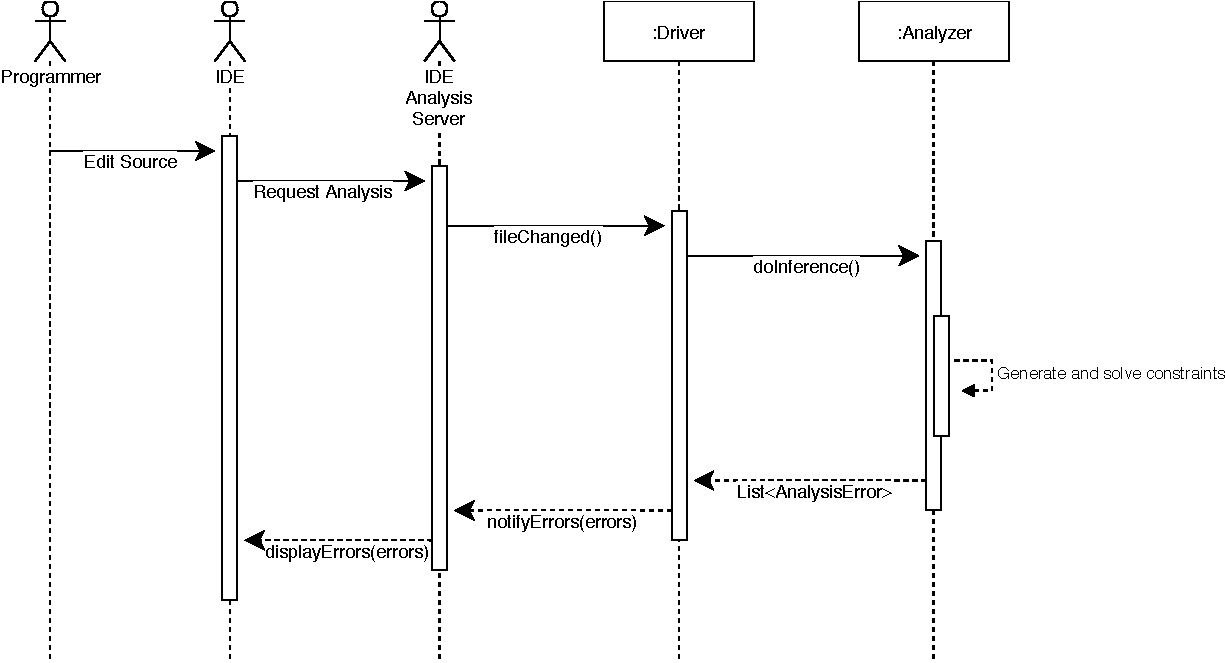
\includegraphics[width=\textwidth]{imagenes/sequence.pdf}
  \caption{Diagrama de secuencia del plugin}
  \label{seq}
\end{figure}

\subsection{Configuración de la extensión}
Para activar el análisis sobre un proyecto, se debe agregar el paquete de la extensión como dependencia al proyecto, y agregar la extensión al archivo de configuración del análisis del proyecto \texttt{analysis\_options.yaml}, ubicado en la raíz del proyecto.

\begin{verbatim}
  analyzer:
    plugins:
      TRNIdart:
        default_core_return: Bot
        default_core_parameter: Bot
\end{verbatim}

Las opciones \texttt{default\_core\_return} y \texttt{default\_core\_parameter} corresponden a las facetas públicas por defecto que tendrán los métodos del core de Dart.

\section{Métricas de la implementación}
El proyecto de la herramienta se denomina \texttt{TRNIdart}~\cite{repo}, por \emph{type-based relaxed noninterference} en Dart, y se divide en tres paquetes, con base en el tutorial oficial de la herramienta Analyzer Plugin~\cite{plugin}.
\clearpage
\begin{itemize}
  \item \texttt{TRNIdart:} Es el paquete que se encarga de inicializar la extensión y donde se define la anotación personalizada de las facetas públicas.
  \item \texttt{TRNIdart\_analyzer:} Es el paquete que contiene la implementación del sistema de inferencia.
  \item \texttt{TRNIdart\_analyzer\_plugin:} Es el paquete que contiene la implementación de la lógica de la extensión.
\end{itemize}
La figura \ref{metricas} muestra la cantidad de líneas de código y de clases que tiene cada paquete, y el total.

\begin{figure}[ht]
  \centering
  \begin{tabular}{l|c|c}
    \textbf{Paquete} & \textbf{Líneas de código} & \textbf{Clases}\\
    \hline
    \texttt{TRNIdart} & 15 & 1\\
    \texttt{TRNIdart\_analyzer} & 2494 & 34\\
    \texttt{TRNIdart\_analyzer\_plugin} & 357 & 7\\
    \hline
    \textbf{Total} & \textbf{2866} & \textbf{42}
  \end{tabular}
  \caption{Cantidad de líneas de código y clases por paquete}
  \label{metricas}
\end{figure}

\section*{Resumen}

En este capítulo se mostraron las librerías de Dart utilizadas en la implementación, la representación de facetas públicas en Dart, los tipos de errores que se generan en las distintas fases del algoritmo de inferencia y los detalles de implementación de la extensión para ambientes de desarrollo. En el siguiente capítulo se muestra la experiencia de programar con facetas públicas y el uso de test unitarios para validar la herramienta.
